%%%%%%%%%%%%%%%%%%%%%%%%%%%%%%%%%%%%%%%%%%%%%%%%%%%%%%%%%%%%%%%%%%%%%%%%%%%%%%%%
\chapter{Overview}

\begin{chapterBody}

% Match the function definitions in the diagram

\begin{figure}[ht]
    \centering
    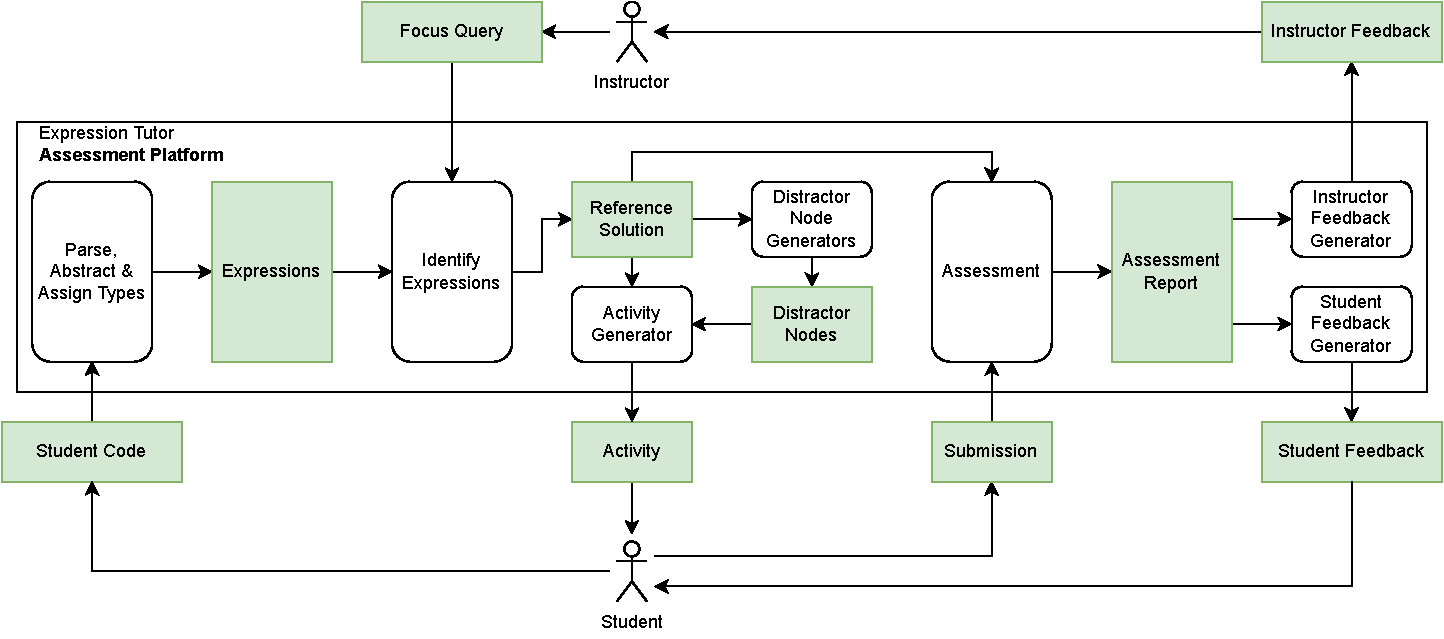
\includegraphics[width=\textwidth]{res/3/et_loop.drawio.pdf}
    \caption{Overview of the system.}
    \label{fig:intro-et-loop}
\end{figure}

In this chapter we describe how instructors and students can use the system 
designed and implemented in this thesis. It serves as an introduction to
subsequent chapters which expand upon the details about design and implementation
of each part of the system.

Originally, it was up to instructors to create, collect and assess activities for
each student.
With the improvements and additions the contributions implemented and detailed in
this document, the data generated by each part of the system can flow into another
component, and finally reaches instructors and students providing them with
useful insights and results.

\textbf{Figure~\ref{fig:intro-et-loop}} highlights how the system operates.
In this figure we find two kinds of elements. White rounded boxes represent
functional components of the system. Green boxes represent data that is either
produced or consumed by components.
The system has two kinds of users: instructors and their students.

We begin with the instructor. 
Usually, in programming courses, students are tasked to complete coding
assignments. The instructor provides them with a template project and
a number of coding exercises they have to implement. The students then
submit their code for assessment and grading.
While devising a coding assignment, the instructor identifies one or
more learning goals that students should achieve by completing said
assignment.
Then, they devise a \textit{focus query} (\textbf{Chapter~\ref{sec:etl}}).
This query is used to select expressions from the source code found in the
submissions of the students. The instructor should design a query so that
it aligns with the learning goals of the coding assignment. This way
the expression selection can effectively be used to assess the code 
comprehension on topics and skills that the instructor deems relevant.

The instructor then proceeds to create an \textit{activity group} on the
Expression Tutor platform (\textbf{Section~\ref{sec:impl-agi-ag}}).
An activity group allows instructors to collect and assess multiple
submissions of Activities submitted by students. The platform offers both
aggregate visualizations and the possibility to view individual submissions
and their assessment. The focus query is also configured into the activity
group. This way, when generating activities that belong to said group, the
system will use the configured query.

The instructor prepares the base template for the code assignment for their
students and includes the configuration for the automatic generation of
Expression Tutor activities. The automatic activity generation is accomplished
by using CI/CD features of a platform such as GitHub 
(\textbf{Section~\ref{sec:impl-aag-gh}}).
For each student, the system generates one or more unique and individual
Activities.

The students are notified of the creation of the Activities that they are tasked
to solve on the Expression Tutor website. Then, the system performs an assessment
of the student's submission (\textbf{Section~\ref{sec:fb-assess}}).
This information is used to provide students with formative feedback
(\textbf{Section~\ref{sec:fb-ff}}) about their submission.

The same information generated by the assessment process is also provided to
instructors, but in a different format compared to that of students.
The activity group created by the instructor at the beginning of the process
collects all the submissions of the multiple different Expression Tutor
activities generated for the same coding assignment.
For each student submission, instructors receive feedback
(\textbf{Section~\ref{sec:fb-sf}}) that helps surface mistakes and common
misconceptions spotted in the submissions. At the same time detailed information
for each of the student's submission is provided. This allows instructors to
review each individual submissions as well.

With the newly gained insights about student's code comprehension regarding the
original learning goal, the instructor can now make more informed decisions for
their next lectures and assignments.

\end{chapterBody}